\documentclass[12pt]{article}

\newlength{\blackoutwidth}
\newcommand{\blackout}[1]
{%necessary comment
  \settowidth{\blackoutwidth}{#1}%necessary comment
  \rule[-0.3em]{\blackoutwidth}{1.125em}%necessary comment
}

\PassOptionsToPackage{usenames,dvipsnames}{xcolor}
\PassOptionsToPackage{colorlinks,linktoc=all}{hyperref}
\usepackage{balance}       % to better equalize the last page
\usepackage{graphics}      % for EPS, load graphicx instead 
\usepackage[T1]{fontenc}   % for umlauts and other diaeresis
\usepackage{txfonts}

\usepackage{color}
\usepackage{booktabs}
\usepackage{textcomp}
\usepackage{cuted}
\usepackage{capt-of}
\usepackage[pdflang={en-US},pdftex]{hyperref}

\title{Comparing Novel Machine-Learning Approaches for Recommending Quality Writing}
\author{Rohan Bansal}
\date{September 2020}

% !TEX root = ../recommending-interesting-writing.tex

% FONTS
%\usepackage[T1]{fontenc}

% Replace default Latin Modern typewriter with its proportional counterpart
% http://www.tug.dk/FontCatalogue/lmoderntypewriterprop/
%\renewcommand*\ttdefault{lmvtt}

%%% OPTION 3 - MTPRO 2 Math + Termes Times + ParaType Sans
\let\myBbbk\Bbbk
\let\Bbbk\relax
\let\bibsep\relax
\let\openbox\relax
\let\proof\relax
\let\endproof\relax
\let\iint\relax
\let\iiint\relax
\let\iiiint\relax
\let\idotsint\relax
%\usepackage{tgtermes}
\usepackage{minted}
\usepackage{amsmath}
\usepackage{blkarray}
% \usepackage[subscriptcorrection,
%             amssymbols,
%             mtpbb,
%             mtpcal,
%             nofontinfo  % suppresses all warnings
%            ]{mtpro2}
% \usepackage{scalefnt,letltxmacro}
% \LetLtxMacro{\oldtextsc}{\textsc}
% \renewcommand{\textsc}[1]{\oldtextsc{\scalefont{1.10}#1}}
% \usepackage[scaled=0.92]{PTSans}

% ICONS
\usepackage{fontawesome}

% CODE

% COLOR
\usepackage[usenames,dvipsnames]{xcolor}
\definecolor{shadecolor}{gray}{0.9}

% SPACING and TEXT
%\usepackage[final,expansion=alltext]{microtype}
%\usepackage[english]{babel}
\usepackage[parfill]{parskip}
\usepackage{afterpage}
\usepackage{framed}
\usepackage{nicefrac}

% EDITING
% line numbering in left margin
\usepackage{lineno}
\renewcommand\linenumberfont{\normalfont
                             \footnotesize
                             \sffamily
                             \color{SkyBlue}}
% ragged paragraphs in right margin
\usepackage{ragged2e}
\DeclareRobustCommand{\sidenote}[1]{\marginpar{
                                    \RaggedRight
                                    \textcolor{Plum}{\textsf{#1}}}}

% Define a paragraph header function
\DeclareRobustCommand{\parhead}[1]{\textbf{#1}~}

% paragraph helper
\DeclareRobustCommand{\PP}{\textcolor{Plum}{\P}~}
\DeclareRobustCommand{\pp}{\textcolor{Plum}{\P}~}

% COUNTERS
\renewcommand{\labelenumi}{\color{black!67}{\arabic{enumi}.}}
\renewcommand{\labelenumii}{{\color{black!67}(\alph{enumii})}}
\renewcommand{\labelitemi}{{\color{black!67}\textbullet}}

% FIGURES
\usepackage{graphicx}
\usepackage[labelfont=bf]{caption}
\usepackage[format=hang]{subcaption}

% TABLES
\usepackage{booktabs}
%\usepackage{dblfloatfix}  % for placing table at bottom of page

% TABLE ALIGNMENT
\usepackage{etoolbox,siunitx}
\robustify\bfseries
\sisetup{detect-weight=true, detect-shape=true, detect-mode=true,
table-format=5.1,
table-number-alignment=center,
separate-uncertainty=true,
input-ignore={,},input-decimal-markers={.}}

% BABEL
% \usepackage{polyglossia}

% BIBLIOGRAPHY
\usepackage[backend=biber, style=numeric-comp]{biblatex}
%\usepackage{natbib}

% ALGORITHMS
\usepackage[algoruled]{algorithm2e}
\usepackage{listings}
\usepackage{fancyvrb}
\fvset{fontsize=\normalsize}

% THEOREMS
\usepackage{amsthm}
\newtheorem{theorem}{Theorem}
% \newtheorem{proposition}[proposition]{Proposition}
\newtheorem{prop}{Proposition}


% TODO
%\usepackage{todo}

% HYPERREF
%\usepackage[colorlinks,linktoc=all]{hyperref}
\usepackage[all]{hypcap}
\hypersetup{citecolor=Violet}
\hypersetup{linkcolor=black}
\hypersetup{urlcolor=MidnightBlue}

% CLEVEREF must come after HYPERREF
\usepackage[capitalize]{cleveref}

% ACRONYMS
\usepackage[acronym,smallcaps,nowarn]{glossaries}
% \makeglossaries

% COLOR DEFINITIONS
\newcommand{\red}[1]{\textcolor{BrickRed}{#1}}
\newcommand{\orange}[1]{\textcolor{BurntOrange}{#1}}
\newcommand{\green}[1]{\textcolor{OliveGreen}{#1}}
\newcommand{\blue}[1]{\textcolor{MidnightBlue}{#1}}
\newcommand{\gray}[1]{\textcolor{black!60}{#1}}

% LISTINGS DEFINTIONS
\usepackage{listings}
\lstdefinestyle{alp_style}{
    commentstyle=\color{OliveGreen},
    numberstyle=\tiny\color{black!60},
    stringstyle=\color{BrickRed},
    basicstyle=\ttfamily\scriptsize,
    breakatwhitespace=false,
    breaklines=true,
    captionpos=b,
    keepspaces=true,
    numbers=none,
    numbersep=5pt,
    showspaces=false,
    showstringspaces=false,
    showtabs=false,
    tabsize=2
}
\lstset{style=alp_style}

% !TEX root = ../set_recommendation.tex

\DeclareRobustCommand{\mb}[1]{\ensuremath{\boldsymbol{\mathbf{#1}}}}
%\DeclareRobustCommand{\mb}[1]{\mathbold{#1}}

\DeclareRobustCommand{\KL}[2]{\ensuremath{\textrm{KL}\left(#1\;\|\;#2\right)}}

\DeclareMathOperator*{\argmax}{arg\,max}
\DeclareMathOperator*{\argmin}{arg\,min}

\newcommand{\yqm}{y_{qm}}
\newcommand{\xum}{x_{um}}
\newcommand{\xuk}{x_{uk}}
\newcommand{\yuk}{y_{uk}}
\renewcommand{\mid}{~\vert~}
\newcommand{\prm}{\:;\:}

\newcommand{\mbw}{\mb{w}}
\newcommand{\mbW}{\mb{W}}

\newcommand{\mbx}{\mb{x}}
\newcommand{\mbX}{\mb{X}}

\newcommand{\mby}{\mb{y}}
\newcommand{\mbY}{\mb{Y}}

\newcommand{\mbz}{\mb{z}}
\newcommand{\mbZ}{\mb{Z}}

\newcommand{\mbI}{\mb{I}}
\newcommand{\mbone}{\mb{1}}

\newcommand{\mbL}{\mb{L}}

\newcommand{\mbtheta}{\mb{\theta}}
\newcommand{\mbTheta}{\mb{\Theta}}
\newcommand{\mbomega}{\mb{\omega}}
\newcommand{\mbOmega}{\mb{\Omega}}
\newcommand{\mbsigma}{\mb{\sigma}}
\newcommand{\mbSigma}{\mb{\Sigma}}
\newcommand{\mbphi}{\mb{\phi}}
\newcommand{\mbPhi}{\mb{\Phi}}

\newcommand{\mbalpha}{\mb{\alpha}}
\newcommand{\mbbeta}{\mb{\beta}}
\newcommand{\mbgamma}{\mb{\gamma}}
\newcommand{\mbeta}{\mb{\eta}}
\newcommand{\mbmu}{\mb{\mu}}
\newcommand{\mbrho}{\mb{\rho}}
\newcommand{\mblambda}{\mb{\lambda}}
\newcommand{\mbzeta}{\mb{\zeta}}

\newcommand\dif{\mathop{}\!\mathrm{d}}
\newcommand{\diag}{\textrm{diag}}
\newcommand{\supp}{\textrm{supp}}

\newcommand{\E}{\mathbb{E}}
\newcommand{\V}{\mathbb{V}}
\newcommand{\bbH}{\mathbb{H}}

\newcommand{\bbN}{\mathbb{N}}
\newcommand{\bbZ}{\mathbb{Z}}
\newcommand{\bbR}{\mathbb{R}}
\newcommand{\bbS}{\mathbb{S}}

\newcommand{\cL}{\mathcal{L}}
\newcommand{\cS}{\mathcal{S}}
\newcommand{\cD}{\mathcal{D}}

\newcommand{\cN}{\mathcal{N}}
\newcommand{\cT}{\mathcal{T}}

\newcommand{\mult}{\textrm{Mult}}
\newcommand{\dirichlet}{\textrm{Dirichlet}}
\newcommand{\Gam}{\textrm{Gamma}}
\newcommand{\Pois}{\textrm{Poisson}}
% !TEX root = recommending-interesting-writing.tex

\newacronym{ELBO}{elbo}{evidence lower bound}
\newacronym{GMM}{gmm}{Gaussian mixture model}
\newacronym{KL}{kl}{Kullback-Leibler}
\newacronym{LDA}{lda}{latent Dirichlet allocation}
\newacronym{SVI}{svi}{stochastic variational inference}
\newacronym{DEF}{def}{deep exponential family}
\newacronym{rfs}{rfs}{\textsc{rankfromsets}}
\newacronym{bert}{bert}{\textsc{bert}}
\newacronym{NLP}{NLP}{natural language processing}
\newacronym{ctpf}{ctpf}{collaborative topic Poisson factorization}

\bibliography{bib}
\begin{document}

\begin{titlepage}
    \begin{center}
        \vspace*{1cm}
            
        \huge
        \textbf{Comparing Novel Machine Learning Approaches for Recommending Quality Writing}
            
        \vspace{0.5cm}

        \vspace{1.5cm}
        
        \vfill
        
        \Large
        \textbf{Research Question: } \\
        \large
        \emph{How do transformer models with pre-contextualized word embeddings compare to set-based recommendation models, such as a dot-product model, in their ability to classify articles on the basis of the "quality" of their writing, as assessed by expert humans?}
            
        \vspace{0.8cm}
            
        \Large
        Word Count: 3998
            
    \end{center}
\end{titlepage}

\tableofcontents
\newpage

\section{Introduction}
This essay is focused on comparing two modern machine learning approaches in their ability to classify and predict “quality” writing. This type of writing can be thought of as the material published in curated newsletters (such as The Browser) or quality-focused publications such as Longform.org. A concept such as quality-writing is inherently subjective due to its opinion-based nature, however, there are some notable aspects that seem to follow through what people typically regard as high-quality work. Pragmatic and unique descriptions, a strong topic and character development, and a logical structure are common keys in the analysis of good writing. Furthermore, scientists have found that content curators often use a very similar process when filtering articles, indicating that there is a programmable science to the art. This leads to the inference (and experiment) presented in this paper as a model with this ability can drastically reduce the workload of these editors while also providing a healthier newsfeed for indpendent consumers. There seems to be a general paucity of serious work in this space, partially because it may be quite difficult to train a machine to understand what we humans would consider fantastic literature and also because finding adequate data can be difficult and expensive. The two approaches considered are \gls{rfs}~\parencite{altosaar2020rankfromsets:} and \acrshort{bert}~\parencite{devlin2019bert:}, both novel machine-learning approaches. The primary method of comparison between the two models will come from their respective recall on the held-out evaluation set. The top 1000 predictions for each model will be considered, and the percentage of true positives will determine the model’s score. Other time and computing constraints will also be discussed throughout to provide enhanced context for all results. Hence, the question: \emph{How do transformer models with pre-contextualized word embeddings compare to set-based recommendation models, such as a dot-product model, in their ability to classify articles on the basis of the "quality" of their writing, as assessed by expert humans?}

\section{Theory}
The concept of machine learning has become more popular for many tasks due to its ability to reduce human error and provide efficient methods for solving real-world problems. Prior to its advent, programming was generally a practice in which a developer gave instructions to a computer and the machine executed the commands it received. In contrast, machine learning teaches a computer to “think” or develop a model on its own that can then be utilized to tackle new situations. For example, classification-based systems, such as those being used in this paper, rely on large amounts of labeled data in the form of a \textbf{training dataset}. \textbf{Labels} refer to the category of each instance in the dataset, so they would be “quality” (0) or “regular” (1) here. The training set is fed to the model in \textbf{batches} (for computational speed and even label splits), where the model uses its \textbf{parameters} to generate predictions for the examples within the batch. These predictions are compared to the actual labels to calculate the \textbf{loss}, which measures the discrepancy between the predictions and intended results. Finally, an \textbf{optimizer} uses \textbf{back-propagation} (calculating the derivative of the final output with respect to each parameter) to update the parameters based on the loss. Machine learning also uses an evaluation and test dataset, which are used to monitor the progress of the model’s parameters. The model generates predictions on the evaluation set with a fixed frequency during training with back-propagation turned off. This allows the researcher to ensure that the model is not over-fitting on the training set, or becoming overly specific to the articles being trained on. Once evaluation performance begins to decrease, the model is used to generate predictions on a test set to get final results on completely new data. The model can then be used to generate new predictions on unlabelled data, such as for the purpose of a recommendation application system that fetches new articles daily. The specific subset of machine learning used in this paper is \gls{NLP} which pertains to text analysis.

\section{Approaches}

\subsection{NLP Fundamentals}
The primary challenge in any text-based modeling approach is the representation of data. A computer cannot comprehend words like humans, so it needs a numeric approach for text analysis. This leads to the idea of using ids to map words~\parencite{nlpfundamentals}. For example, consider the sentence: “John went to the park.”. We can easily construct a basic dictionary for the words in this sentence and map them to a unique id as such: 

$\{"john" : 0, "went" : 1, "to" : 2, "the" : 3, "park" : 4\}$

\subsubsection{One-Hot Encoding}
This process could also occur for labels/categories that need to be numerically represented, such as colors or publications. However, there is a very obvious issue with this approach when using it on unordered data without obvious spatial relationships. This type of map tells the model that “park” is more important, or weighted more heavily, than “john”. If the model calculates averages, it will find the average of the words “went” and “the” to equal “to”. These types of relationships are obviously fraught and would cause major errors in the model’s effectiveness. To mitigate this problem, researchers developed the concept of one-hot encoding, which essentially binarizes the process of mapping items to their numeric representations~\parencite{harris_harris_2015}. A matrix is generated with dimensions length of items in entry X length of total dictionary for each example. Each row of the matrix has a single one and all other entries are zero to represent the single word. Using the above example, our sentence representation would become:

\[\begin{bmatrix}
1 & 0 & 0 & 0 & 0\\
0 & 1 & 0 & 0 & 0\\
0 & 0 & 1 & 0 & 0\\
0 & 0 & 0 & 1 & 0\\
0 & 0 & 0 & 0 & 1\\
\end{bmatrix}\]

Although this mitigates the earlier concerns, there are a variety of disadvantages to this approach. Firstly, the creation of such sparse matrices for each entry in the dataset, which can span millions of entries, is inefficient for storage purposes. It is also plagued by the “curse of dimensionality” as each category/word appends an entire dimension to the matrix~\parencite{bellman_1954}. Finally, the adding of items to the dictionary would lead to changing the representations for all previous words. Aside from the structural issues, this approach lacks interpretability. As the items are fed into the model, the one-hot encoded matrix tells the user nothing about the relationship between words. It also breaks down any order of words, which is required for models such as \acrshort{bert}.

\subsubsection{Embedding Vectors}
These major problems with one-hot encoding led to the development of embeddings and vectorized representations of words in natural language processing. The fundamental premise of word embeddings is the concept that each word maps to a unique n-sized vector of a single dimension. Thus, words can be mapped to ids as they were above, and a separate mapping of ids to vectors can be utilized to convert each word into a corresponding mathematical representation. The embeddings are obviously not directly interpretable by humans, as they capture latent qualities of the word as the model is trained, however embeddings offer a significant advantage over one-hot encoding in their ability to offer comprehensible representations. Similar words will be found to be spatially contiguous. The relationship between words can also be calculated directly through cosine similarity, which is essentially the arccosine of the dot product of two vectors normalized by their magnitudes. The most famous example of this type of interpretability is the mathematical relationship \textbf{king - man + woman = queen} which can be graphically observed in Figure 1, produced by \textcite{king_man_woman_queen}: 

\begin{figure}[h]
\centering
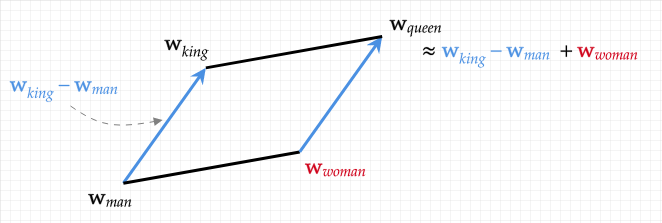
\includegraphics[width=0.8\textwidth]{fig/king-man-woman-queen.png}
\caption{Spatial representation of king - man + woman = queen}
\label{fig:king_man_woman_queen_pic}
\end{figure}

This then allows for each example in the dataset to be represented as a unidimensional list of word ids, which can then be mapped to their corresponding vectors when being processed by the model. The data storage advantages are obvious, as each entry becomes easily stored as a single dense list instead of the highly-sparse matrices generated by one-hot encoding. Thus, because of both the data-related and interpretability advantages offered by embeddings, they were utilized for both of the tested models.

\subsection{RankFromSets (RFS)}
\gls{rfs} was proposed by \textcite{altosaar2020rankfromsets:} and was initially used for the task of recommending meals to users based on their prior data of favorite food combinations. I used a slightly modified version in my research. The recommender system utilizes an unordered set of attributes to represent each individual item. An inner-product architecture parametrizes the classifier:
\begin{equation}
\label{eq:inner-product}
  f\left(q, x_m\right) = \theta_p^\top\left(\frac{1}{|x_m|}\sum_{j\in x_m}
  \beta_j\right) + \frac{1}{|x_m|}\sum_{j\in x_m}
  \gamma_j\, .
\end{equation}

Each aspect of \Cref{eq:inner-product} has an intuitive definition:

$\theta_p^\top$: the publication embedding for publication $p$. Here, there is only one 
publication (that of quality writing), however, the simplicity of the model allows for 
scalability to generate predictions for multiple publications.

$x_m$: the set of unique word tokens in the article. Because the model does not take 
positional relationships of words into account, the ordered set of tokens can be used to   
mitigate the effects of the repetition of frequently used words such as \emph{the, and, a}.

$\beta_j$: the latent quality of each word in the set represented by $x_m$. This is a vector representing the word’s “meaning” that is updated during training. These vectors are summed across the set and normalized by word-list length.

$\gamma_j$: the scalar bias of each word in the set represented by $x_m$. These are used to prevent overfitting and account for qualities of a word that were not represented within the embedding vector (such as frequency). These were also summed and normalized.

Normalization of the sums of biases and vector representations is done to prevent article length from playing an outsized role in predictions. The vector sum is then multiplied with the “quality” writing publication embedding, which has identical dimensions. The normalized word biases are added to generate the final output of the function.

The final probability is defined as:
\begin{equation}
\label{eq:sigmoid_rfs}
p(\yqm = 1 \mid q, m) = \sigma\left( f \left (q, x_m\right) \right)\, 
\end{equation}

In \Cref{eq:sigmoid_rfs}, $\sigma$ is the sigmoid function, defined by:
\begin{equation}
\label{eq:sigmoid}
S(x) = \frac{1}{1 + e^{-x}}, 
\end{equation}

$\sigma$ takes an input and generates a final probability between $0$ and $1$, which is then rounded to get a positive or negative prediction~\parencite{svetoslav_2015}. The implementation of the model is presented through a custom subclass of the PyTorch Module~\parencite{NEURIPS2019_9015} and~\parencite{altosaar2020rankfromsets:}:

\begin{minted}{python}
class RankFromSets(nn.Module):
    def __init__(self, n_pubs, n_attrs, emb_size):
        super().__init__()
        self.emb_size = emb_size
        self.publication_embeddings = nn.Embedding(n_pubs, emb_size)
        self.publication_bias = nn.Embedding(n_pubs, 1)
        self.attribute_emb_sum = nn.EmbeddingBag(n_attrs,
                                                emb_size, mode="mean")
        self.attribute_bias_sum = nn.EmbeddingBag(n_attrs, 1, mode="mean")

    # this method resets default parameters to normal distribution
    def reset_parameters(self):
        for module in [self.publication_embeddings, self.attribute_emb_sum]:
            scale = 0.07
            nn.init.uniform_(module.weight, -scale, scale)
        for module in [self.publication_bias, self.attribute_bias_sum]:
            nn.init.zeros_(module.weight)

    def forward(self, publications, word_attributes, attribute_offsets):
        # get publication embedding and bias
        publication_emb = self.publication_embeddings(publications)
        publication_bias = self.publication_bias(publications)
        # get sum of attribute embedding vectors
        article_and_attr_emb = self.attribute_emb_sum(
            word_attributes, attribute_offsets
        )
        # get sum of attribute biases
        attr_bias = self.attribute_bias_sum(word_attributes, attribute_offsets)
        # dot-product of pub_emb and attr_emb sum
        inner_prod = (publication_emb * article_and_attr_emb).sum(-1)
        # add biases to result and return final logits
        logits = inner_prod + attr_bias.squeeze() + publication_bias.squeeze()
        return logits
\end{minted}

\subsection{Bidirectional Encoder Representations from Transformers (BERT)}
\acrshort{bert} was proposed by \textcite{devlin2019bert:} and obtained state-of-the-art results on a variety of NLP-related tasks, including sentence classification and next word predictions. The model is predicated on the concept of transformers, which were released in 2017 and provided a method for ensuring that the sequential nature of text data was accounted for in machine learning models ~\parencite{transformers:}. Prior to their advent, the primary method for encoding spatial word relationships was through the use of Recurrent Neural Networks (RNN). They input tokens sequentially and create a new latent state based on the previous $n-1$ tokens combined with the recently inputted $n$th token. The general input process is depicted by ~\textcite{olah_2015}:

\begin{figure}[h]
\centering
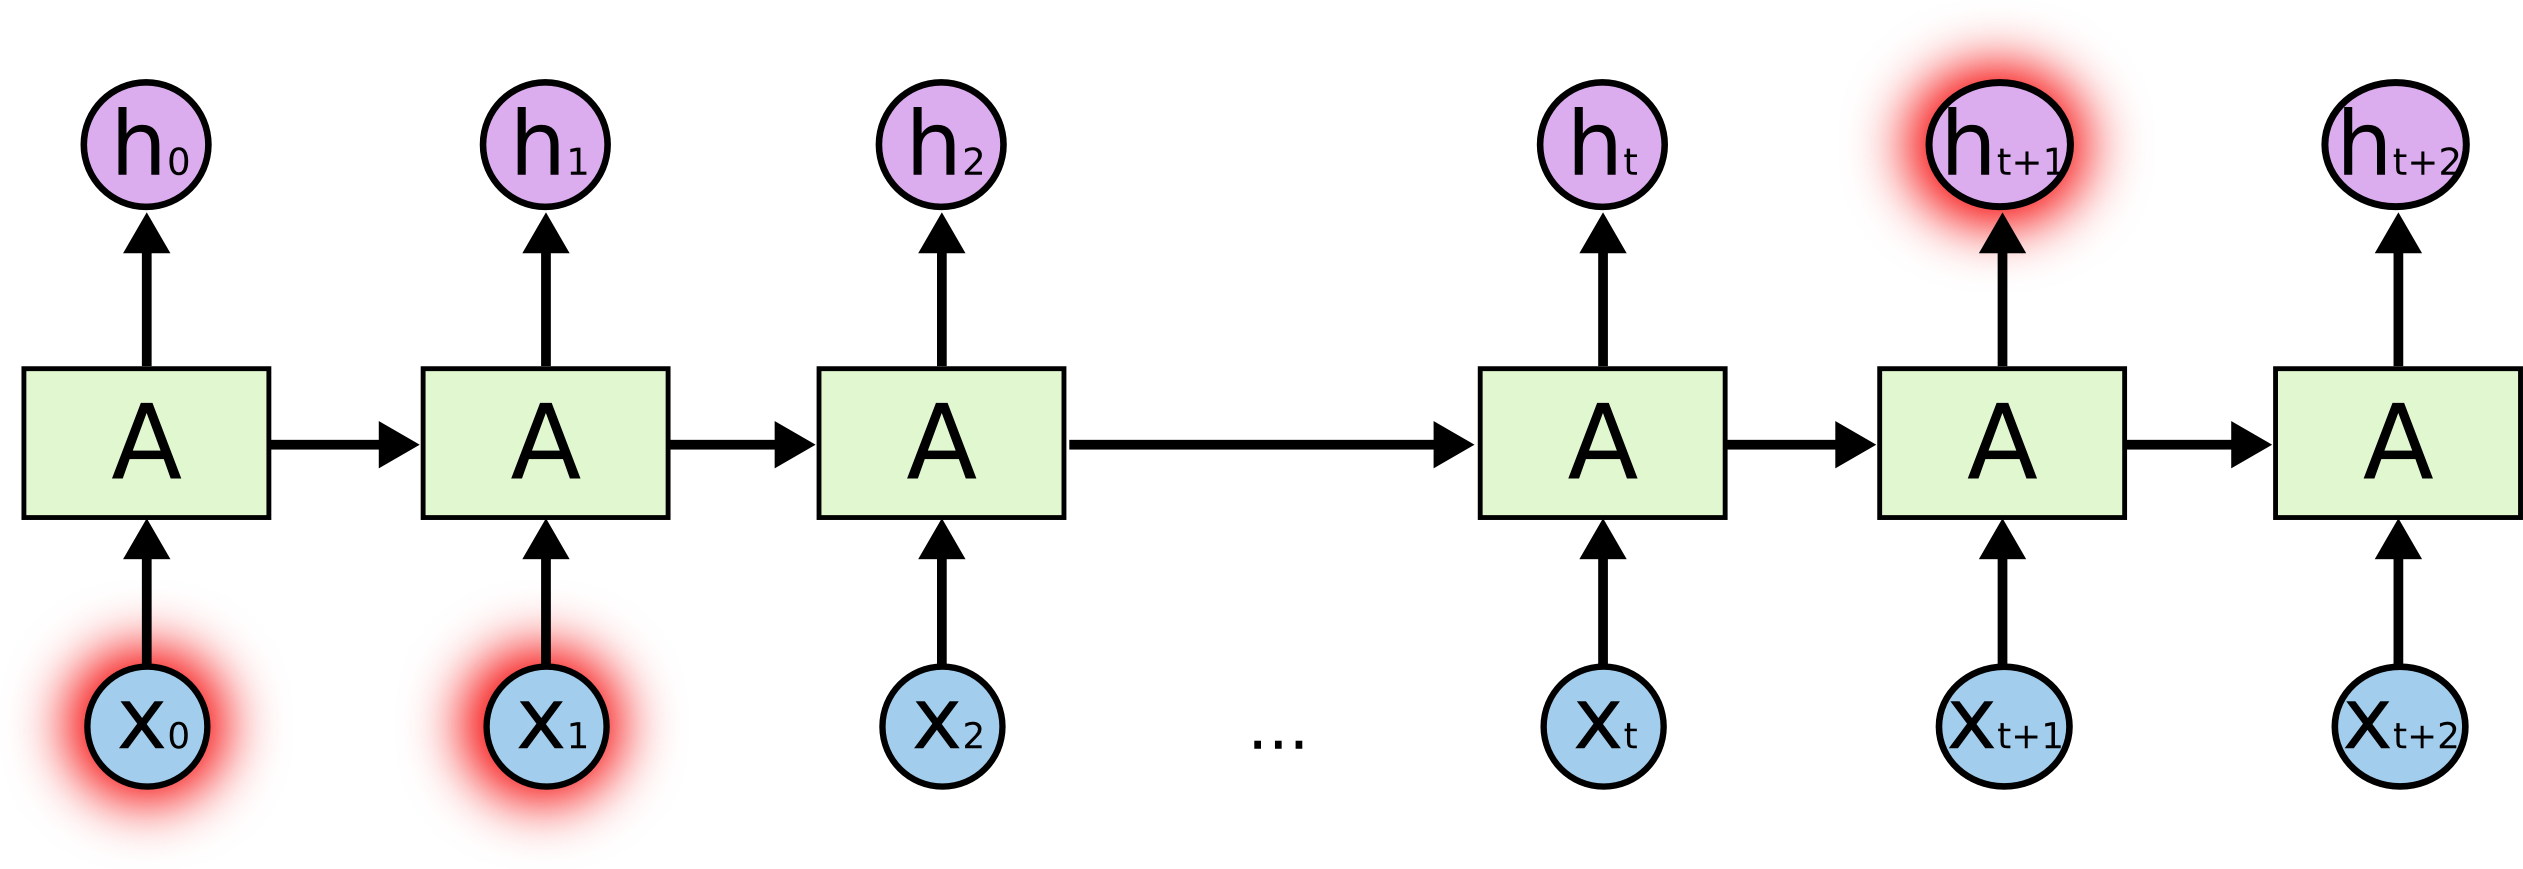
\includegraphics[width=0.8\textwidth]{fig/rnn.png}
\caption{RNN sequencing example (displays sequential input handling and state updating)
}
\label{fig:rnn}
\end{figure}

There were a variety of problems that hindered this approach, including a lack of concrete connection between early and later words of a sequence. Additionally, as only a single hidden state was stored after each token was added, the weight (or visibility) of the beginning of the input could often become hidden and difficult for the model to recover ~\parencite{hochreiter1997long}. 
For example, if a model is being trained to translate from English to Spanish, it can be reasonably assumed that the first few words of the English input have a strong correlation to the correct beginning tokens of the Spanish Output. However, the model only contains the final latent state of the input, thus making it difficult for it to correctly decipher the beginning of the Spanish translation. Transformers were created to offer an alternative to this process, and they rely on a concept called attention and involve two components, an encoder and a decoder ~\parencite{transformers:}. As \acrshort{bert} relies only on encoders, this paper will focus exclusively on them.

\subsubsection{Encoders}
An encoder consists of two sub-layers, a self-attention layer that calculates the relation of each token to other tokens in the same input and a feed-forward network which works like a normal multi-layer perceptron. Self-attention is essentially the concept of helping the model comprehend the relationships of words to other tokens in the input. For example, consider the sequence: \\

\textbf{The money has gone missing. Where is it?} \\

For a human, it would be fairly easy to understand that \textbf{it} is referring to the \textbf{money}. But for a machine, it can be much more difficult to gather these types of contextual clues, especially if the corresponding words are separated ~\parencite{hochreiter1997long}. Thus, self-attention generates “scores” for each input token with every other token (including itself) which helps it understand the relationships that are not explicitly present in the direct translation. \\

The encoder takes the raw embedding sequence as input which is passed to the self-attention layer. The embeddings are slightly modified before being fed to the model however. It is important for the computer to have some sense of the spatial relationships between words (the relative distances) to help with the positional aspect of the sequence. Thus, the model utilizes learned positional embeddings, which are the same size as the word embeddings themselves ~\parencite{devlin2019bert:}. These positional vectors are added to the token vectors to create the real input:

\begin{figure}[h]
\centering
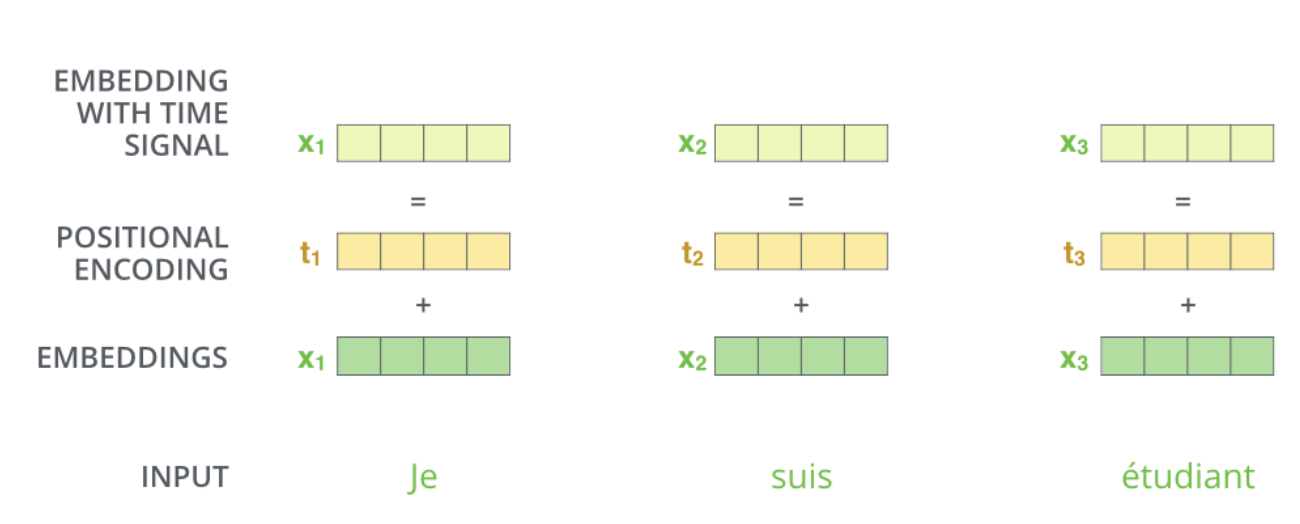
\includegraphics[width=0.8\textwidth]{fig/positional_encodings.png}
\caption{The basic addition of positional encodings to the input vectors before being fed to the model~\parencite{alammar_2018}.
}
\label{fig:positional_encodings}
\end{figure}

This layer then utilizes three matrices to generate a key, value, and query for each input token. For \acrshort{bert}, the embedding vectors are of length $768$, and each of these matrices has dimensions $768 \times 64$. For each token, the embedding vector is multiplied by the three matrices to get the key, query, and value vectors which each have a length of $64$. Then, the dot-product between the query vector and each token’s key is calculated to generate a score. This can be observed here:

\begin{figure}[h]
\centering
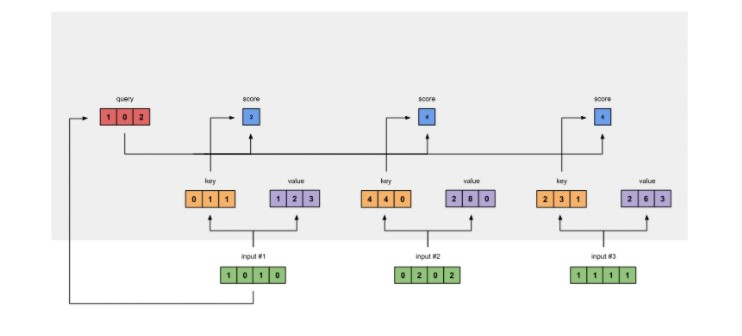
\includegraphics[width=0.8\textwidth]{fig/first_encoder_step.jpg}
\caption{Initial score generation for first token by taking a dot-product between the query vector and the key vectors for each token~\parencite{karim_2019}.)
}
\label{fig:first_encoder_step}
\end{figure}

The scores are then normalized with a $softmax$ function, defined by:
\begin{equation}
\label{eq:softmax}
S(y_i) = \frac{e^{y_i}}{\sum_{j\in y}e^{y_j}}, 
\end{equation}

\Cref{eq:softmax} takes a list of numbers and normalizes them into a probability distribution based on the exponential values of the inputs ~\parencite{bengio_goodfellow_courville_2017}. These normalized scores are multiplied with the corresponding value vectors, which then are summed element-wise to get a final score for the token:

\begin{figure}[H]
\centering
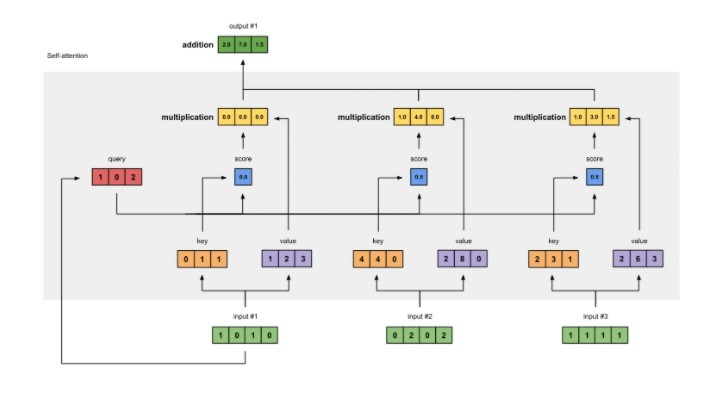
\includegraphics[width=0.8\textwidth]{fig/second_encoder_step.jpg}
\caption{The SoftMax function is applied to the initial score, then multiplied with the value vectors. The results are then summed to generate a final output for the first token.~\parencite{karim_2019}.
}
\label{fig:second_encoder_step}
\end{figure}

This process is performed for each input token and is vectorized for faster computation. Transformers are able to utilize this process multiple times per encoder to generate what is known as multi-headed attention. In the case of \acrshort{bert}, this process is done $8$ separate times, each with a different key, query, and value matrix to get $8$ vectors of length $64$ for each input token. This makes the attention layer even more powerful and allows for more concrete connections to be encoded between words ~\parencite{transformers:}. However, the feed-forward layer is not expecting each token to have multiple associated vectors, thus these outputs must be combined first before sending. To alleviate this problem, the vectors are all concatenated together to create a vector of length 512 $(8 \times 64)$, then multiplied with another parameter matrix of dimensions $512 \times 768$, to return to the original embedding size of $768$ ~\parencite{devlin2019bert:}, which is outlined here:

\begin{figure}[H]
\centering
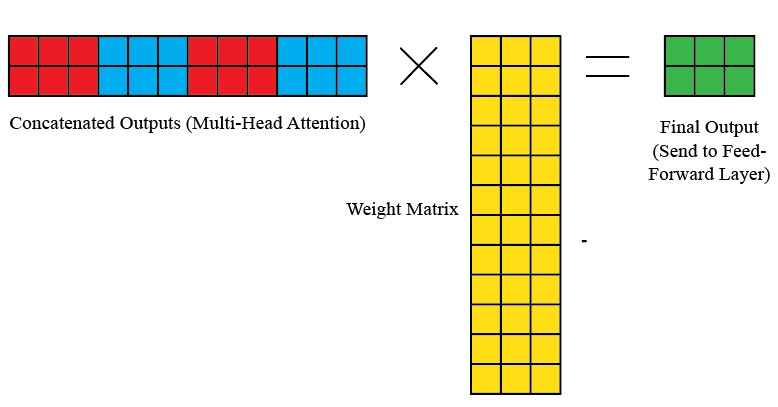
\includegraphics[width=0.8\textwidth]{fig/multi-head.jpg}
\caption{The outputs are concatenated as above then multiplied with the weighted matrix that is updated throughout training to get a final output with a 768 long vector for each token.
}
\label{fig:multi_head_attention}
\end{figure}

The overall attention process can be summarized as the following:
\begin{equation}
\label{eq:attention}
Attention\left(Q, K, V\right) = softmax\left(\frac{QK^\top}{\sqrt{d_k}}\right)V, 
\end{equation}

\Cref{eq:attention} outlines the attention function for a $(Q,K,V)$ value tuple. The results of the query and key product are divided by the square root of the size of the vectors (8 for~\acrshort{bert}) to normalize the outputs before applying softmax ~\parencite{transformers:}.

This attention layer output is then passed to the fully-connected feed forward neural network, which takes inputs of length 768 and returns an output of identical size based on a non-linear activation function as such:

\begin{figure}[H]
\centering
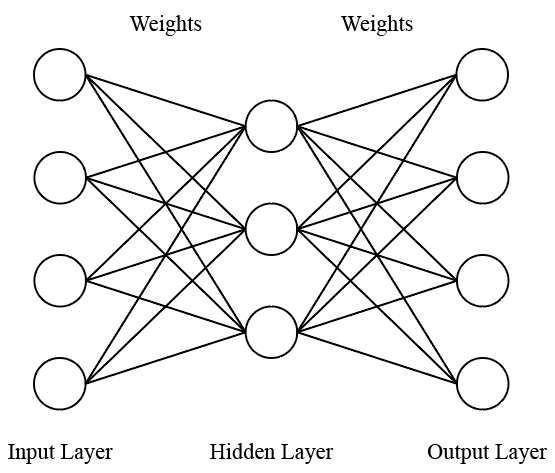
\includegraphics[width=0.8\textwidth]{fig/full_neural.png}
\caption{A sample fully-connected feed forward network with a hidden layer}
\label{fig:neural-network}
\end{figure}

The workings of a neural network have been extensively documented throughout machine learning literature, thus they will not be discussed in detail. However, the basic premise is very similar to the workings of \acrshort{rfs}, where a dot-product is calculated with learned weights, and then passed through an activation function, such as $\sigma$ \parencite{lecun2015deep}.

\subsubsection{General Working}
\acrshort{bert} employs 12 of these encoders, with both self-attention and feed forward components, stacked on top of each other. Because the model is being used for classification, another final neural network is placed on top that takes the outputs of the encoders and generates a single probability for the entry \parencite{sun2019finetune}.

\section{Hypothesis/Applied Theory}
Based on the information presented about both approaches, it is very clear that \acrlong{rfs} is more flexible than \acrshort{bert}. \acrshort{bert} utilizes over 100 million parameters and thus requires significantly more computing power and GPU memory to be run even on smaller datasets. However, this large gap in parameters and empirical evidence suggests that \acrshort{bert} will outperform \gls{rfs} on practically any NLP task as it is able to better fit unique datasets ~\parencite{devlin2019bert:}.

This experiment will analyze both the time taken to train the models on the same data, but also the recall/performance of the models. Recall will be tested by looking at the percentage of true positives in the top 1000 predictions of each model. I hypothesize that \acrshort{bert} will have a moderate advantage in recall performance, but \acrshort{rfs} will overfit on the data many magnitudes faster.

\section{Data Collection and Processing}
The majority of the work necessary for training machine learning models pertains to the actual data being trained on. Many steps are involved in acquiring proper data and cleaning it in a manner that makes training both conducive and effective.

\subsection{Collection}
I began by collecting data from longform.org and longreads.com, which are both publications that scour the web for quality content. The crawling/scraping scripts I wrote and used can be seen in~\Cref{appendix:crawling} and~\Cref{appendix:scraping}. I then asked the CEO of The Browser for his content and he graciously provided access to the company’s archives (refer to~\Cref{appendix:permission}). These articles were combined to be positive examples. To collect negative data, I began with scraping a few major news sites (Vox, Guardian). I then decided to scrape specific publications that frequently appear in the quality writing locations, as these would provide a better test of the models' ability to draw a distinction from content that is actually hand-picked for its writing style. This included sources such as Rolling Stone and Smithsonian Magazine who both focus on longform content. I also decided to use the Fake News Corpus which provides nearly 9 million articles from various fringe parts of the Internet, including hate speech, genuine fake news, and conspiracy theories. These were generally used for non-training purposes to ensure that the model was not susceptible to "bad" content.

\subsection{Cleaning}
The majority of the cleaning and processing was done via the direct crawling/scraping scripts. JSON files were generated for each publication, which included fields for publication, text, and links. The only major caveat with this type of scraping is the possibility for certain sites to detect the script and send back an error message. For this step, I manually checked a few articles from each publication scrape to make sure that proper content was being received by the request. I also filtered out articles that were under 75 words in length as these were primarily error messages or not technically full-length articles.

\subsection{Preparation}
After collection, the text and publication fields had to be mapped to ids for the model. For publications, I mapped all of the quality content I had collected to publication id 0. The remaining publication ids were essentially irrelevant as the model was only relying on the embedding vector for publication 0 to generate predictions. The text needed to be mapped to the corresponding tokens. The tokenizer library from huggingface made this process easy, as it allows for a simple input of a normal sequence of text (in the way that the article content was saved) and generates a dataset of both tokenized words and the corresponding ids which can be observed here:

\begin{figure}[H]
\centering
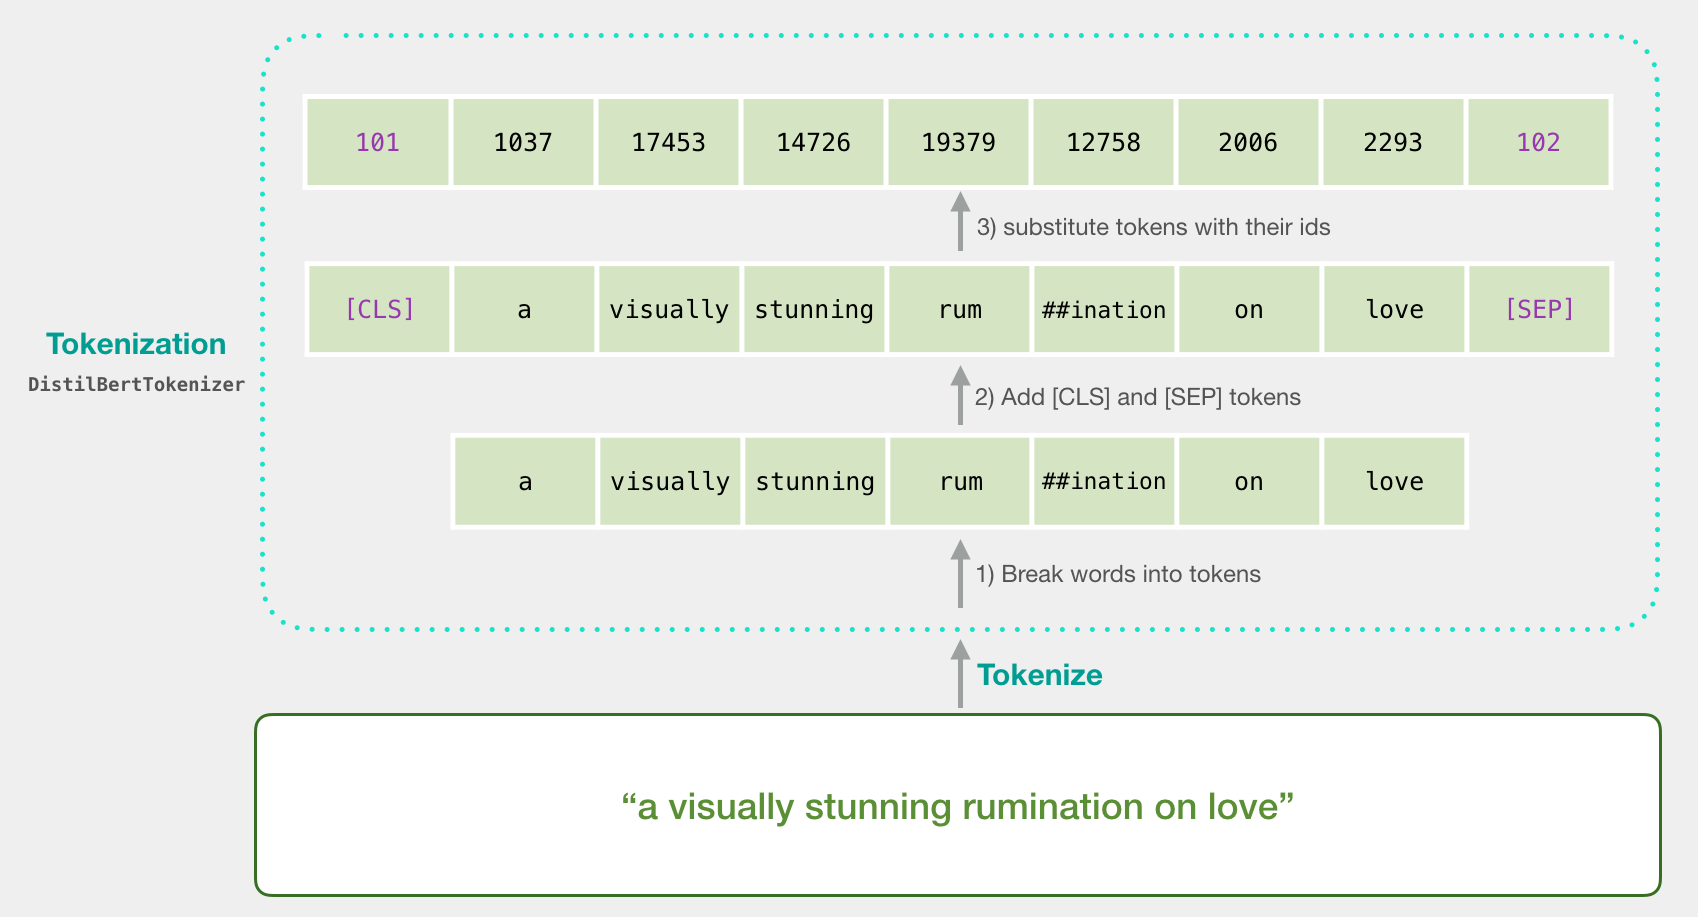
\includegraphics[width=0.8\textwidth]{fig/tokenization.png}
\caption{Full Scale Tokenization Example, where an English sentence is converted to tokens~\parencite{alammar_2019}.
}
\label{fig:tokenization}
\end{figure}

In order to limit the need for separate data files for both approaches, I chose not to add any other pre-processing to the text fields, such as removing duplicates or adding custom tokens. \acrshort{bert} relies on the spatial relationship between words in the sequence, and thus I wanted to maintain that order and only make structural changes when needed (see~\Cref{appendix:processing}). This was done in the actual training scripts themselves to reduce overhead. 

\section{Experiments}
For both experiments, 15$\%$ of the data was held out as a test and validation set each. The  exact breakdowns of the sets can be seen in Appendix .Recall was utilized to measure performance ($\%$ of true positives in top 10 and 1000 of predictions). Gridsearchs were used to run models with all posible combinations of chosen configurations. The models were also evaluated with early-stopping (training was stopped when model exhibited maximum performance on the validation set) to prevent over-fitting.

\subsection{Experimental Setup: RankFromSets}
\acrshort{rfs} was run using RMSProp optimizer~\parencite{tieleman2012lecture} with a momentum of 0.9 and a gridsearch was done over learning rates of $\{10^{-2}, 10^{-3}, 10^{-4}, 10^{-5}\}$, embedding sizes of $\{10, 25, 50, 100, 500, 1000\}$, and a decision of whether or not to pre-initialize the model with BERT embeddings. The basic training loop is shown here:
\begin{minted}{python}
for step, batch in enumerate(cycle(train_loader)):
    # turn to training mode and calculate loss for backpropagation
    torch.enable_grad()
    model.train()
    optimizer.zero_grad()
    publications, articles, word_attributes, attribute_offsets, real_labels = batch
    publication_set = [args.target_publication] * len(real_labels)
    publication_set = torch.tensor(publication_set, dtype=torch.long)
    publication_set = publication_set.to(device)
    articles = articles.to(device)
    word_attributes = word_attributes.to(device)
    attribute_offsets = attribute_offsets.to(device)
    logits = model(publication_set, articles, word_attributes, attribute_offsets)
    L = loss(logits, labels)
    L.backward()
    optimizer.step()
    running_loss += L.item()
\end{minted}

\subsection{Experimental Setup: BERT}
As \acrshort{bert} already comes "pre-trained", I fine-tuned it to the collected data with the AdamW optimizer and a linear learning rate scheduler with warm up steps according to best practices, as outlined by ~\textcite{devlin2019bert:} and ~\textcite{wolf2019huggingfaces}. The model used a batch size of 32, and articles had maximum length of 512 tokens. A grid search was performed over learning rates of $\{2, 3, 4, 5\} \times 10^{-5}$, warmup steps of $\{10^2, 10^3, 10^4\}$, and total training steps $\{10^2, 10^3, 10^4, 10^5\} \times 5$. The basic training loop is shown here:
\begin{minted}{python}
for step, batch in enumerate(cycle(train_loader)):
    # turn to training mode and calculate loss for backpropagation
    torch.enable_grad()
    optimizer.zero_grad()
    word_attributes, attention_masks, word_subset_counts, real_labels = batch
    word_attributes = word_attributes.to(device)
    attention_masks = attention_masks.to(device)
    logits = model(word_attributes, attention_masks)[0]
    logits = torch.squeeze(logits)
    L = loss(logits, labels)
    L.backward()
    if args.clip_grad:
        nn.utils.clip_grad_norm_(model.parameters(), 1.0)
    optimizer.step()
    scheduler.step()
    running_loss += L{}.item()
\end{minted}

\subsection{Quantitative Evaluation}
The best performing models from both approaches were chosen, and were evaluated via recall on the test set.
% !TEX root = ../proceedings.tex
\begin{table}[h]
\centering
\begin{tabular}{lSS}
\toprule
Recommendation Model & \multicolumn{1}{c}{Recall @ 1000 (\%)}
\\
\midrule
\acrlong{rfs} &  \bfseries 53.1\\
\acrshort{bert} & 46.6 \\
\bottomrule
\end{tabular}
% BERT 466/1000
% rankfromsets 531/1000
% \vspace{1ex}
\caption{\gls{rfs} outperforms \acrshort{bert} in an offline evaluation on the test dataset when predicting which articles would be featured at The Browser}
\label{tab:recall}
\end{table}

Additionally, the time taken to train the models is shown:

% !TEX root = ../recommending-interesting-writing.tex
\begin{figure}[h]
  \centering
  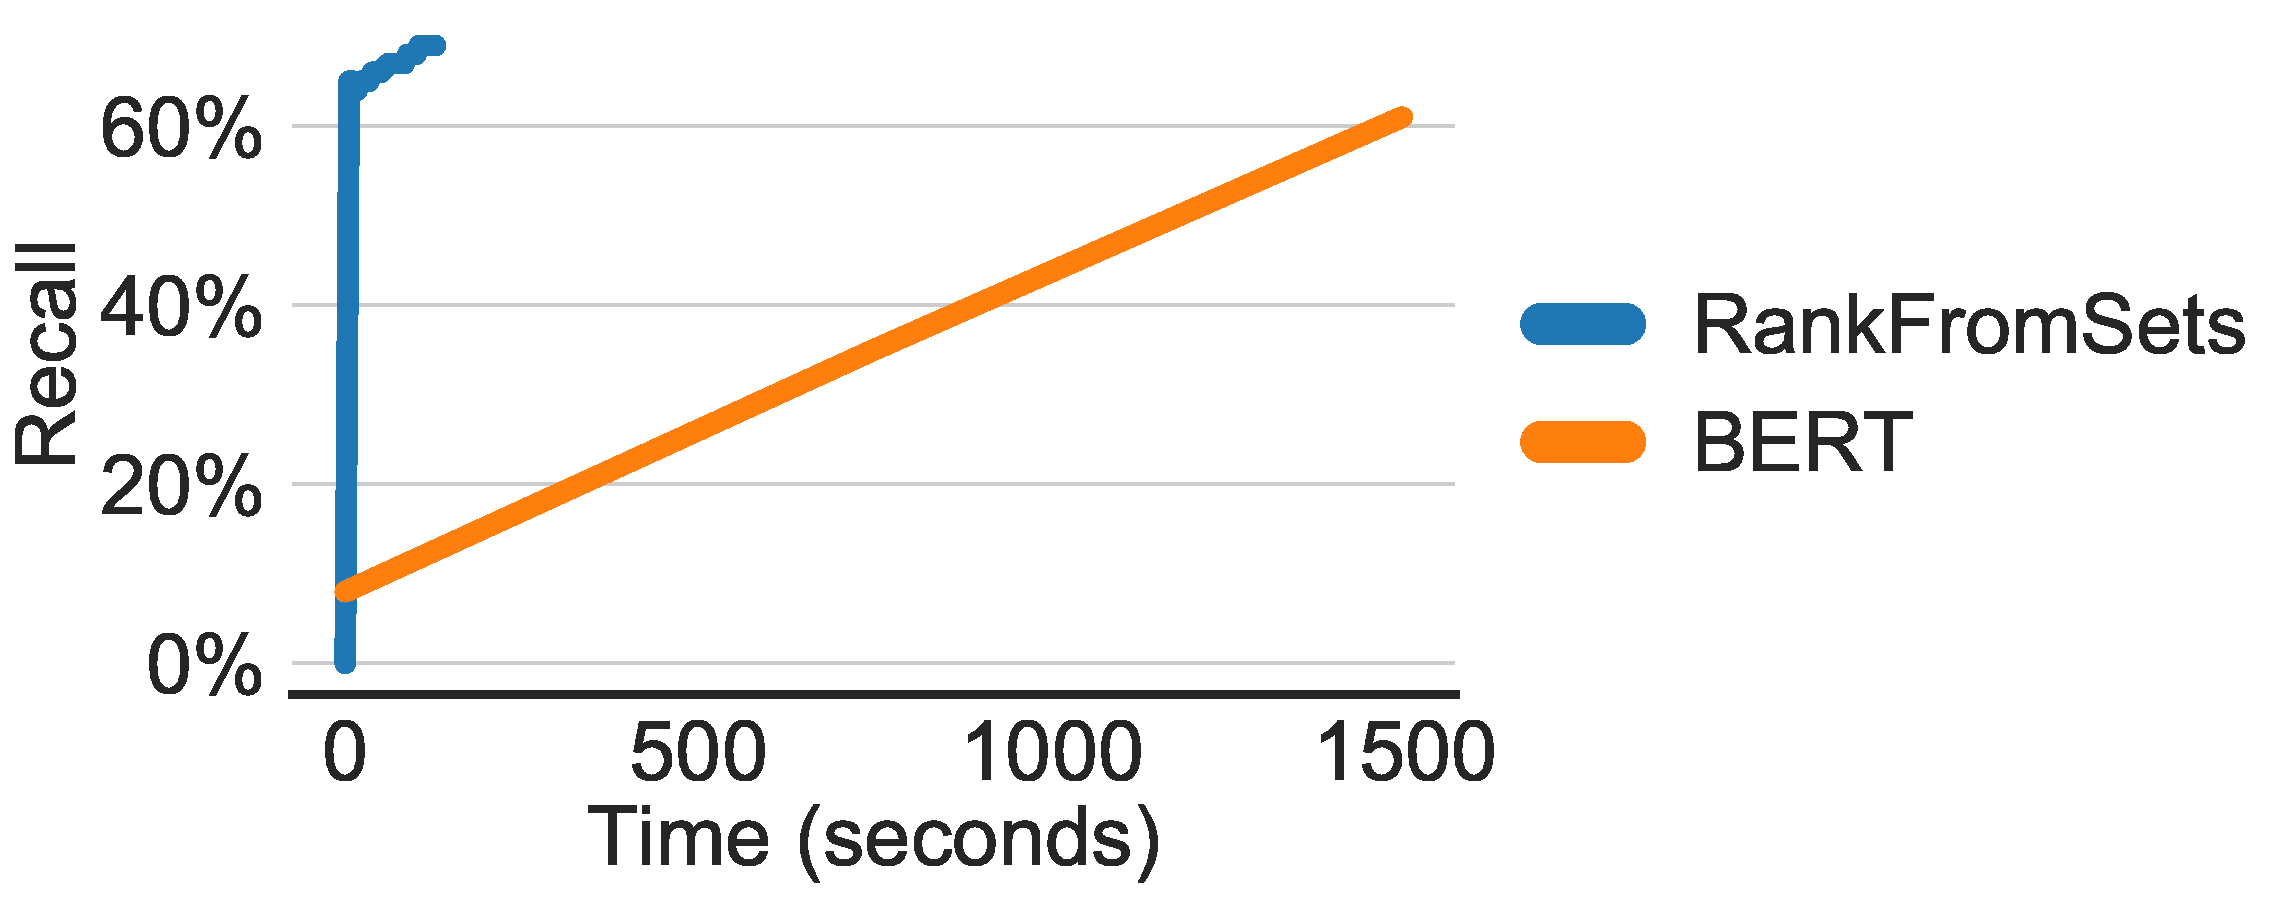
\includegraphics[width=0.95\linewidth]{fig/training-recall}
  \caption{\acrshort{rfs} achieves better performance faster than \acrshort{bert} in terms of validation recall during training.}
  \label{fig:training-recall}
\end{figure}

\section{Discussion}
My hypothesis that \acrshort{bert} would outperform \acrshort{rfs} was proved to be incorrect, as \acrshort{rfs} actually performed over $6\%$ better as shown in Table~\ref{tab:recall}. However, my other inference that \acrlong{rfs} would overfit faster was shown to be correct by Figure~\ref{fig:training-recall}.

The results were obviously statistically significant, which can easily be deduced by the breakdown of the datasets (Refer to Appendix~\ref{appendix:data-info})
. Based on this data distribution of the test set, a completely random sorting of the articles would result in an anticaptory recall @ 1000 of $0.15\%$ or roughly 2 true positives. The performance of both models was significantly greater than this baseline, indicating that the models were able to learn intrinsic qualities of the text which allowed for the generation of improved predictions on untrained data. However, the difference between the two models' performance is still ambiguous and could simply be due to random error, something which was indicated by the qualitiatative analysis of the predictions by editors at The Browser. Despite this, even comparable results by \acrshort{rfs} indicate a better result than \acrshort{bert}, due to the drastically reduced training and prediction time and the simplistic mathematical framework.


I was, however, intrigued by my initial hypothesis being incorrect, as \acrshort{bert} should theoretically have outperformed \acrshort{rfs}. There were a few possible explanations. Firstly, machine learning approaches sometimes struggle on certain tasks because of the nature of the dataset, so it is possible that \acrshort{bert} was simply unable to fit the data due to an inherent mathematical hindrance in its workings, although this is unlikely~\parencite{domingos2012few}. It is also possible that \acrshort{bert} overfit the training set in an atypical manner. Because of \acrshort{bert}'s inherent complexity, it can be prone to overfitting a dataset due to the assumption of more complicated relationships between the variables and labels. In contrast, \acrlong{rfs} assumed a simple, linear relationship which requires more data to overfit~\parencite{domingos2012few}. It is also possible that there is no direct causational relationship between the words of an article and its "quality", thus the relationships learned by both models were specific only to the dataset chosen. This is also unlikely, as the performance seen was significantly higher than random, however it is a common issue with machine-learning. Finally, \acrshort{bert} typically requires huge loads of data to effectively train, due to its 100 million+ parameters. There is a chance that the training data was simply not large enough for BERT to effectively fit on~\parencite{gonzlezcarvajal2020comparing}.

For future work, it would be important to introduce regularization into the training to further penalize incorrect predictions. This may hinder \acrshort{rfs}' ability, but could boost \acrshort{bert}. Collecting more data could also provide more insight into whether a lack of examples contributed to the final results.

\section{Conclusion}
The purpose of this experiment was to compare two modern machine-learning approaches to NLP in their ability to recommend writing. The theoretical aspects of both models were explored, including the mathematical framework, and gridsearchs were run to determine the best-performing models. It is difficult to draw a direct conclusion in this type of exeriment because of the limited dataset, and the other potential limitations discussed above.

However, when answering the initial research question, \acrlong{rfs} outperformed \acrshort{bert} in recall at 1000 on the test set and generated better results significantly faster. A novel set-based dot-product approach was able to suggest "high-quality" writing at a rate much higher than random. \acrshort{rfs} can also be implemented in an online application or command-line tool to help readers and curators filter large amounts of new articles to the more relevant and interesting reads.

\printbibliography
\cleardoublepage
\appendix
\section{Code Base}
\label{appendix:code-base}
All code utilized in this project can be found at https://github.com/rohanbansal12/extended\_essay. Both approaches, \acrlong{rfs} and \acrshort{bert}, have their own folders in the repository. Crawling/Scraping scripts can be found in the data-collection folder. The files used to build this paper in \LaTeX\ are found in the EE folder. I have included certain examples and relevant scripts throughout the paper and appendices. 

\section{Crawling Scripts}
\label{appendix:crawling}
A few sample crawling scripts that were utilized have been included.
\subsection{Longform.org Crawling Script}
\begin{minted}{python}
@dataclass_json
@dataclass
class LongformArticleUrl:
    url: str
    title: str
    source: str

class WriteThread(Thread):
    def __init__(self, queue: Queue, *args, **kwargs):
        super().__init__(*args, **kwargs)
        self.queue = queue
	def run(self):
        with open(OUTPUT_FILE, 'a') as output_file:
            output_file.write("[\n")
            first_entry = True
			while True:
			    article = self.queue.get()
				if article is None:
			        output_file.write("\n]")
			        break
				article_json = article.to_json(indent=4)
				if first_entry:
			        first_entry = False
			    else:
			        output_file.write(",\n")
				output_file.write(article_json)

class ScrapeThread(Thread):
    def __init__(self, chunk, queue: Queue, *args, **kwargs):
        super().__init__(*args, **kwargs)
        self.chunk = chunk
        self.queue = queue
	def run(self):
        for i in self.chunk:
            try:
                print(f'Getting articles from list page {i}')
                article_list_page = get(f"{BASE_URL}{i}")
                soup = BeautifulSoup(article_list_page.text, "html5lib")
                articles = soup.find_all('article', 
                    {'class': 'post--single'})
                for article in articles: 
                    link = article.find('a', 
                        {'class': 'post__link'})
                    title = article.find('span', 
                        {'class': 'post__title__highlight'})
                    source = article.find('a', 
                        {'class': 'post__permalink'})
                    print(link)
                    if (title is None or 
                        title.string is None or 
                        source is None):
                        continue
                    article_url = LongformArticleUrl(url=link['href'], 
                        title=str(title.string.strip()) or '', 
                        source=source['href'])
                    self.queue.put(article_url)
            except Exception as e:
                print(f'Something went wrong when scraping: {e}')
                print("------------------------------------------")
\end{minted}
\subsection{Vox Crawling Script}
\begin{minted}{python}
@dataclass_json
@dataclass
class VoxArticleUrl:
    url: str
    title: str
    month: int
    year: int

YEARS = [str(month) for month in range(2014,2020)]
MONTHS = [str(month) for month in range(1,13)]

class WriteThread(Thread):
    def __init__(self, queue: Queue, *args, **kwargs):
        super().__init__(*args, **kwargs)
        self.queue = queue

    def run(self):
        with open(OUTPUT_FILE, 'a') as output_file:
            output_file.write("[\n")
            first_entry = True
            while True:
                article = self.queue.get()
                if article is None:
                    output_file.write("\n]")
                    break
                article_json = article.to_json(indent=4)
                if first_entry:
                    first_entry = False
                else:
                    output_file.write(",\n")
                output_file.write(article_json)


class ScrapeThread(Thread):
    def __init__(self, chunk, queue: Queue, *args, **kwargs):
        super().__init__(*args, **kwargs)
        self.chunk = chunk
        self.queue = queue
    def get_urls(self, year, month):
        page = 1
        while True:
            sleep(1)  # Prevent rate limiting
            print(f'Getting articles for {year}-{month}, page {page}')
            return_data = get(f"{BASE_URL}/{year}/{month}/{page}", 
                headers={'Accept': 'application/json'})
            if return_data.status_code != 200:
                print(f"Received status {return_data.status_code}")
                if return_data.status_code != 429:
                    return
                else:
                    sleep(10)
            else:
                page = page + 1
                response = return_data.json()
                soup = BeautifulSoup(response['html'], 
                    "html5lib")
                yield soup
                if not response['has_more']:
                    break
    def run(self):
        for year, month in self.chunk:
            try:
                for html in self.get_urls(year, month):
                    h2s = html.find_all('h2')
                    for h2 in h2s:
                        a = h2.find('a')
                        title = a.string
                        url = a['href']
                        print(title,url)
                        vox_url = VoxArticleUrl(title=str(title), 
                            url=str(url), 
                            month=int(month), 
                            year=int(year))
                        self.queue.put(vox_url)
            except Exception as e: # Best effort
                print(f'Something went wrong when scraping: {e}')
\end{minted}

\section{Scraping Scripts}
\label{appendix:scraping}
The majority of the scraping utilized the same code for all sources, in contrast to the crawling scripts, which were based on the specific HTML layout of the websites. I did utilize an alternative method for difficult to scrape sites, and both are presented here.
\subsection{Vanilla Scraping Script}
\begin{minted}{python}
import json
from dataclasses import dataclass, field
from dataclasses_json import dataclass_json
from datetime import datetime
from newspaper import Article
from bs4 import BeautifulSoup
from typing import List
from queue import Queue
from threading import Thread

@dataclass_json
@dataclass
class LongformArticle:
    title: str = ''
    text: str = ''
    url: str = ''
    source: str = ''

class WriteThread(Thread):
    def __init__(self, queue: Queue, *args, **kwargs):
        super().__init__(*args, **kwargs)
        self.queue = queue

    def run(self):
        with open(OUTPUT_FILE, 'a') as output_file:
            output_file.write("[\n")
            first_entry = True
            while True:
                article = self.queue.get()
                if article is None:
                    output_file.write("\n]")
                    break
                article_json = article.to_json(indent=4)
                if first_entry:
                    first_entry = False
                else:
                    output_file.write(",\n")
                    output_file.write(article_json)


class ScrapeThread(Thread):
    def __init__(self, urls, queue: Queue, *args, **kwargs):
        super().__init__(*args, **kwargs)
        self.urls = urls
        self.queue = queue
    @staticmethod
    def scrape(url):
        article = Article(url['url'])
        article.download()
        article.parse()
        soup = BeautifulSoup(article.html, 'lxml')
        ga = LongformArticle()
        ga.url = url['url']
        ga.title = url['title']
        ga.text = article.text
        ga.source = url['source']
        return ga
    def run(self):
        for url in self.urls: 
            try:
                print(f"scraping {url['url']}")
                article = ScrapeThread.scrape(url)
                self.queue.put(article)
            except Exception as e: # Best effort
                print(f'ScrapeThread Exception: {e}')
\end{minted}

\section{Data Processing}
\label{appendix:processing}
I created an Articles class that made dataset handling easy. It includes a built-in mapping function (map\_items), in addition to other methods, such as sampler creations, that were utilized in the rest of the experiment.
The majority of the work necessary for training machine learning models pertains to the actual data being trained on. Many steps are involved in acquiring proper data and cleaning it in a manner that makes training both conducive and effective.

\subsection{Collection}
I began by collecting data from longform.org and longreads.com, which are both publications that scour the web for quality content. The crawling/scraping scripts I wrote and used can be seen in~\Cref{appendix:crawling} and~\Cref{appendix:scraping}. I then asked the CEO of The Browser for his content and he graciously provided access to the company’s archives (refer to~\Cref{appendix:permission}). These articles were combined to be positive examples. To collect negative data, I began with scraping a few major news sites (Vox, Guardian). I then decided to scrape specific publications that frequently appear in the quality writing locations, as these would provide a better test of the models' ability to draw a distinction from content that is actually hand-picked for its writing style. This included sources such as Rolling Stone and Smithsonian Magazine who both focus on longform content. I also decided to use the Fake News Corpus which provides nearly 9 million articles from various fringe parts of the Internet, including hate speech, genuine fake news, and conspiracy theories. These were generally used for non-training purposes to ensure that the model was not susceptible to "bad" content.

\subsection{Cleaning}
The majority of the cleaning and processing was done via the direct crawling/scraping scripts. JSON files were generated for each publication, which included fields for publication, text, and links. The only major caveat with this type of scraping is the possibility for certain sites to detect the script and send back an error message. For this step, I manually checked a few articles from each publication scrape to make sure that proper content was being received by the request. I also filtered out articles that were under 75 words in length as these were primarily error messages or not technically full-length articles.

\subsection{Preparation}
After collection, the text and publication fields had to be mapped to ids for the model. For publications, I mapped all of the quality content I had collected to publication id 0. The remaining publication ids were essentially irrelevant as the model was only relying on the embedding vector for publication 0 to generate predictions. The text needed to be mapped to the corresponding tokens. The tokenizer library from huggingface made this process easy, as it allows for a simple input of a normal sequence of text (in the way that the article content was saved) and generates a dataset of both tokenized words and the corresponding ids which can be observed here:

\begin{figure}[H]
\centering
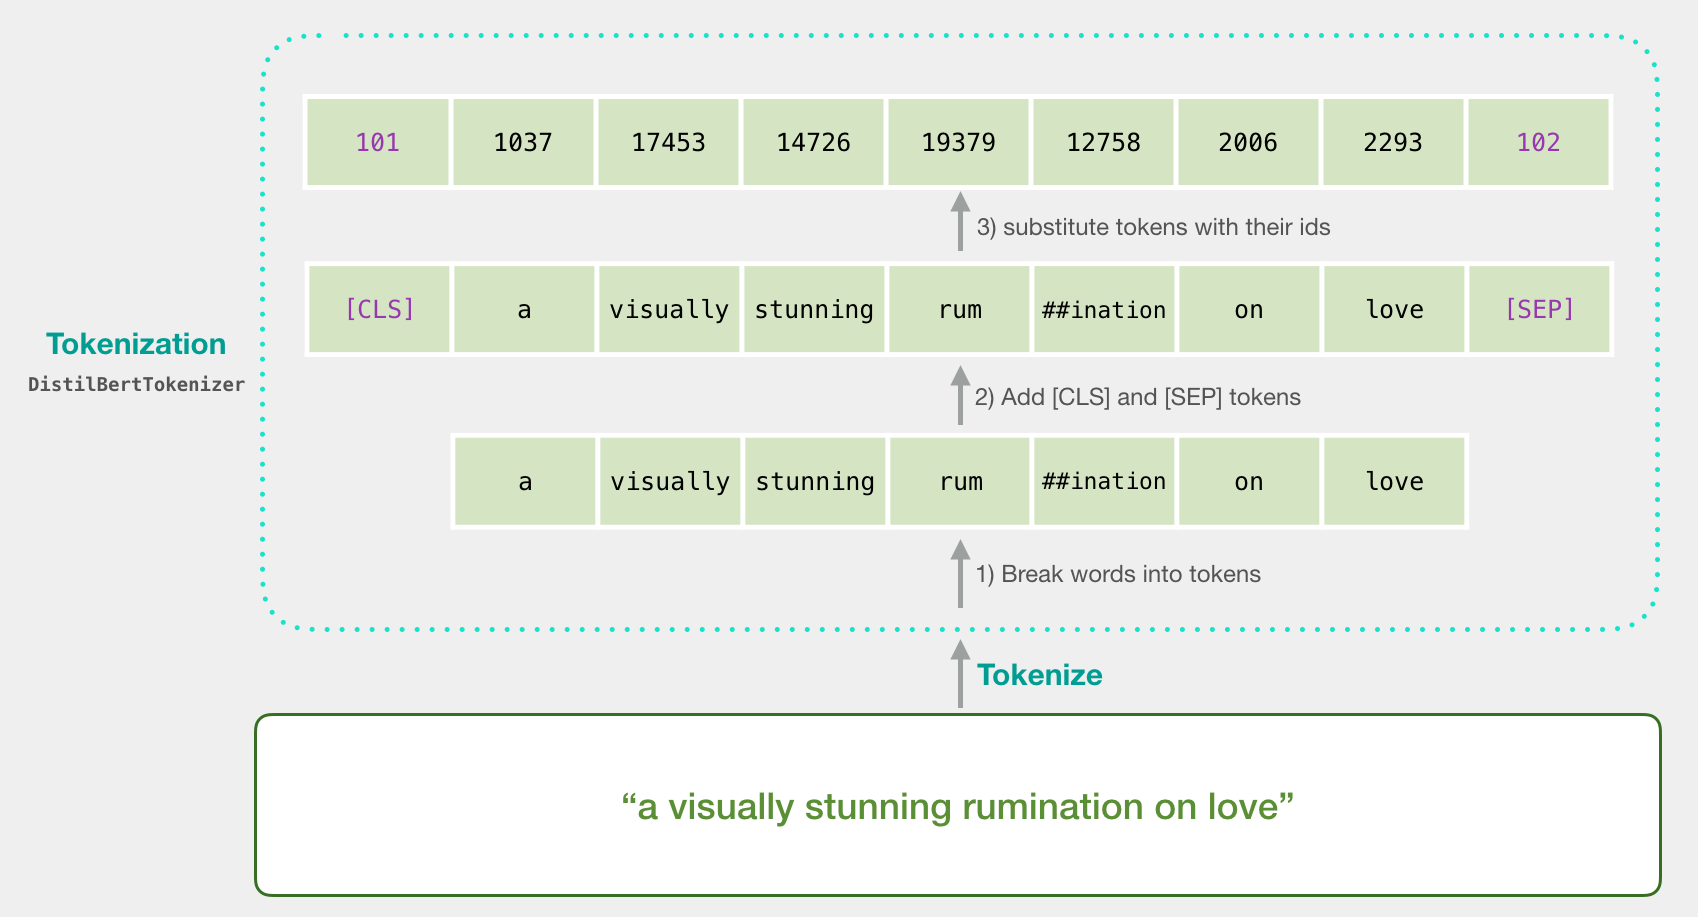
\includegraphics[width=0.8\textwidth]{fig/tokenization.png}
\caption{Full Scale Tokenization Example, where an English sentence is converted to tokens~\parencite{alammar_2019}.
}
\label{fig:tokenization}
\end{figure}

In order to limit the need for separate data files for both approaches, I chose not to add any other pre-processing to the text fields, such as removing duplicates or adding custom tokens. \acrshort{bert} relies on the spatial relationship between words in the sequence, and thus I wanted to maintain that order and only make structural changes when needed (see~\Cref{appendix:processing}). This was done in the actual training scripts themselves to reduce overhead. 

\section{Data Distribution}
\label{appendix:data-info}
The scraped data was converted into train, test, validation sets through a $70\%, 15\%, 15\%$ split. The fake-news corpus was then added only to the validation and test sets, making them much larger and more negative heavy.
% !TEX root = ../proceedings.tex
\begin{table}[h]
\centering
\begin{tabular}{|c|c|c|c|}
\hline
\multicolumn{4}{|c|}{Data Distribution} \\
\hline
Dataset & Total Length & $\#$ of Positive Examples & $\#$ of Negative Examples\\
\hline
Train & 100797 & 18598 & 82199 \\
Validation & 272447 & 4039 & 268348 \\
Test & 272448 & 4049 & 268399 \\
\hline
\end{tabular}
% BERT 466/1000
% rankfromsets 531/1000
% \vspace{1ex}
\caption{Dataset Breakdowns for training, test, and validation sets.}
\label{tab:data-breakdown}
\end{table}

\section{Training Scripts}
\label{appendix:training-scripts}
A collection of some of the most important training scripts that were utilized when performing the experiments.
\subsection{Evenly-Split Batch Generator}
For improved stability of the training process and because of the skewed nature of the datasets, I chose to feed in batches that had an even number of positive and negative labels. To do this, I created a subclass of the PyTorch Sampler \parencite{NEURIPS2019_9015}.
\begin{minted}{python}
import torch
import numpy as np
import torch.nn as nn

# Create batches with even splits
# positive samples in first half and negative examples in second half
class BatchSamplerWithNegativeSamples(torch.utils.data.Sampler):
    def __init__(self, pos_sampler, neg_sampler, batch_size, items):
        self._pos_sampler = pos_sampler
        self._neg_sampler = neg_sampler
        self._items = items
        assert (
            batch_size % 2 == 0
        ), "Batch size must be divisible by two for negative samples."
        self._batch_size = batch_size

    def __iter__(self):
        batch, neg_batch = [], []
        neg_sampler = iter(self._neg_sampler)
        for pos_idx in self._pos_sampler:
            batch.append(pos_idx)
            neg_idx = pos_idx
            # keep sampling until we get a true negative sample
            while self._items[neg_idx] == self._items[pos_idx]:
                try:
                    neg_idx = next(neg_sampler)
                except StopIteration:
                    neg_sampler = iter(self._neg_sampler)
                    neg_idx = next(neg_sampler)
            neg_batch.append(neg_idx)
            if len(batch) == self._batch_size // 2:
                batch.extend(neg_batch)
                yield batch
                batch, neg_batch = [], []
        return

    def __len__(self):
        return len(self._pos_sampler) // self._batch_size

\end{minted}

\subsection{RankFromSets Batched Predictions}
\begin{minted}{python}
@torch.no_grad()
def calculate_batched_predictions(batch, model, device, target):
    model.eval()
    (publications, articles, word_attributes, 
    attribute_offsets, real_labels) = batch
    publication_set = [target] * len(real_labels)
    publication_set = torch.tensor(publication_set, dtype=torch.long)
    publication_set = publication_set.to(device)
    articles = articles.to(device)
    word_attributes = word_attributes.to(device)
    attribute_offsets = attribute_offsets.to(device)
    logits = model(publication_set, articles, 
    			   word_attributes, attribute_offsets)
    final_logits = logits.cpu().numpy()
    return final_logits
\end{minted}

\subsection{BERT Batched Predictions}
\begin{minted}{python}
@torch.no_grad()
def calculate_batched_predictions(batch, model, device, target):
    model.eval()
    (word_attributes, attention_masks, 
    word_subset_counts, real_labels) = batch
    word_attributes = word_attributes.to(device)
    attention_masks = attention_masks.to(device)
    logits = model(word_attributes, attention_mask=attention_masks)[0]
    final_logits = np.squeeze(logits.cpu().numpy())
    return final_logits
\end{minted}

\subsection{Recall Calculation}
\begin{minted}{python}
@torch.no_grad()
def calculate_recall(
    dataset, indices, recall_value=1000, 
    target_publication, version, writer, step,
):
    rev_indices = indices[::-1]
    correct_10 = 0
    correct_big = 0
    for i in range(recall_value):
        if dataset[rev_indices[i]]["model_publication"] == target_publication:
            if i < 10:
                correct_10 += 1
            correct_big += 1
    print(f"{version} Performance: Step - {step}")
    print(f"Top 10: {correct_10*10} %")
    print(
        f"Top {str(recall_value)}: {(correct_big*100)/recall_value} %"
    )
    print("--------------------")
    writer.add_scalar(f"{version}/Top-10", correct_10, step)
    writer.add_scalar(f"{version}/Top-{recall_value}", correct_big, step)
    return correct_big
\end{minted}

\section{Permission Email}
\label{appendix:permission}
\subsection{Email Sent to Mr. Uri Bram of The Browser}

Hello Mr. Bram,

I am currently working on a machine-learning computer science paper for school. My goal is to compare models in their ability to predict "quality" writing. There is a general scarcity in terms of positive data in this space, and I was wondering if I could utilize your Browser archives. The data will not be published or utilized in any external manner. 

Thanks in advance, \\
\blackout{Rohan}

\subsection{Permission Received from Mr. Uri Bram of The Browser}

Dear \blackout{Rohan},

Thank you so much for your kind email. It sounds like a great project and we would be happy for you to use the Browser archive. Please let me know if I can be of any further assistance.

Best,

Uri Bram
CEO, The Browser Ltd
\end{document}{}
